% Аналитический раздел
\chapter{Аналитический раздел}

В этом разделе проводится анализ предметной области медицинской клиники, формализуется задача разработки базы данных и приложения, выделяются основные сущности и роли пользователей, а также рассматриваются модели данных, пригодные для хранения и обработки медицинской информации.

\section{Анализ предметной области и существующих решений}

Предметная область охватывает деятельность медицинской клиники, в которой требуется хранить сведения о пациентах и врачах, управлять расписанием приема, оформлять запись, проводить прием, рассчитывать стоимость услуг и регистрировать оплаты. Особенностью данной области является необходимость одновременного соблюдения медицинских, организационных и финансовых требований: система должна быть удобной для повседневной работы персонала, но при этом не должна допускать конфликтов по времени, произвольного изменения стоимости услуг и нарушения согласованности между приемом, счетом и оплатой.

Основные проблемы предметной области можно сформулировать следующим образом:
\begin{itemize}
    \item расписание врача задается интервалами доступности и должно исключать пересечение записей;
    \item запись на прием выполняется несколькими пользователями одновременно, поэтому система должна корректно работать при конкурентном доступе;
    \item стоимость медицинских услуг может изменяться во времени, следовательно, требуется хранение истории цен;
    \item завершение приема должно приводить к формированию счета на основе реально оказанных услуг, а не только предварительной записи;
    \item доступ к операциям должен различаться в зависимости от роли пользователя.
\end{itemize}

Среди существующих решений можно выделить три класса систем: специализированные медицинские информационные системы, универсальные CRM-платформы и ручной учет в электронных таблицах. Медицинские информационные системы обычно уже содержат расписание врачей, карточки пациентов, приемы и оплату услуг, но их внутренняя структура часто закрыта, а настройка под конкретные правила клиники требует внедрения готового продукта. Универсальные CRM удобны для учета клиентов и задач, однако медицинские сущности в них приходится выражать через сделки, статусы и пользовательские поля. Электронные таблицы подходят для простого учета, но не защищают данные от ошибок при одновременной работе нескольких пользователей.

Сравнение существующих решений приведено в таблице~\ref{tab:solutions}.

\begin{table}[ht]
    \centering
    \caption{Сравнение существующих решений для автоматизации клиники}
    \label{tab:solutions}
    \scriptsize
    \renewcommand{\arraystretch}{1.08}
    \begin{tabularx}{\textwidth}{|>{\raggedright\arraybackslash}p{3.2cm}|>{\raggedright\arraybackslash}X|>{\raggedright\arraybackslash}X|>{\raggedright\arraybackslash}X|}
        \hline
        Критерий & Медицинские ИС & Универсальные CRM & Электронные таблицы \\
        \hline
        Хранение расписания врачей & Штатный календарь врача и кабинета. & Календарь и задачи без медицинских правил. & Таблица расписания, заполняемая вручную. \tabularnewline
        \hline
        Запрет пересечения записей & Обычно реализован на уровне системы. & Требует настройки правил или доработки. & Контролируется пользователем вручную. \tabularnewline
        \hline
        История цен услуг & Поддерживается через прайс-листы и периоды действия. & Может храниться в пользовательских полях. & Есть риск перезаписи старых значений. \tabularnewline
        \hline
        Проведение приема & Есть карточка приема, диагноз и рекомендации. & Не является базовой сущностью CRM. & Обычно ведется на отдельных листах. \tabularnewline
        \hline
        Поддержка счетов и оплат & Счета, строки счетов и статусы оплаты. & Частично через сделки, счета или интеграции. & Ручной расчет и ручное изменение статусов. \tabularnewline
        \hline
        Ролевая модель & Пациент, врач, администратор и другие роли. & Роли интерфейса без явной модели прав БД. & Ограничение доступа только к файлу или листу. \tabularnewline
        \hline
        Аудит и проверка данных & Журнал действий и отчеты. & Частично зависит от настроек CRM. & Проверка затруднена, ошибки легко внести вручную. \tabularnewline
        \hline
    \end{tabularx}
\end{table}
\normalsize

В рамках курсовой работы необходимо разработать собственную базу данных, которая хранит данные медицинской клиники и поддерживает основные операции: запись на прием, проведение приема, формирование счетов и регистрацию оплат. При этом часть правил должна контролироваться самой базой данных: запрет пересечения записей врача, хранение истории цен, пересчет состояния счета и разделение прав доступа.

\section{Формализация задачи}

В ходе выполнения курсовой работы необходимо разработать базу данных для хранения информации о пациентах, врачах, специальностях, медицинских услугах, расписании приема, записях, приемах, счетах и оплатах медицинской клиники. Также необходимо спроектировать и разработать приложение, которое будет предоставлять интерфейс для взаимодействия с базой данных.

Необходимо предусмотреть возможность регистрации пациентов, просмотра расписания врачей и прайс-листа, записи пациента на прием, отмены записи, проведения приема врачом, внесения результатов приема, формирования счета по оказанным услугам и регистрации оплаты. Для разных категорий пользователей требуется реализовать собственный набор прав.

Пациент должен иметь возможность работать со своими записями и просматривать доступную информацию. Врач должен иметь возможность просматривать свое расписание, проводить прием и вносить его результаты. Администратор должен иметь возможность управлять справочниками, расписанием, записями пациентов и оплатами.

При разработке необходимо обеспечить корректность хранения данных. Запись на прием не должна пересекаться с уже занятыми интервалами врача, стоимость услуги должна сохраняться с учетом истории изменения цен, а состояние счета должно обновляться после изменения оказанных услуг или оплат. В качестве основной СУБД используется PostgreSQL, для кэширования часто запрашиваемых данных используется Redis.

\section{Формализация данных и описание структуры базы данных}

На основании формализации задачи выделены следующие основные сущности предметной области: пользователь, роль, специальность, врач, пациент, услуга, цена услуги, интервал доступности врача, отсутствие врача, запись на прием, прием, оказанная услуга, счет и оплата. Для описания связи многие-ко-многим между врачами и услугами используется отдельная сущность связи.

На основании выделенных сущностей построена ER-диаграмма, представленная на рисунке~\ref{fig:er-diagram}. Диаграмма отражает основные сущности предметной области и связи между ними: пользователи связаны с ролями через промежуточную таблицу, врачи привязаны к специальностям и услугам, записи на прием связывают пациента с врачом и услугой, а завершение приема порождает счет и оплаты.

\begin{figure}[H]
    \centering
    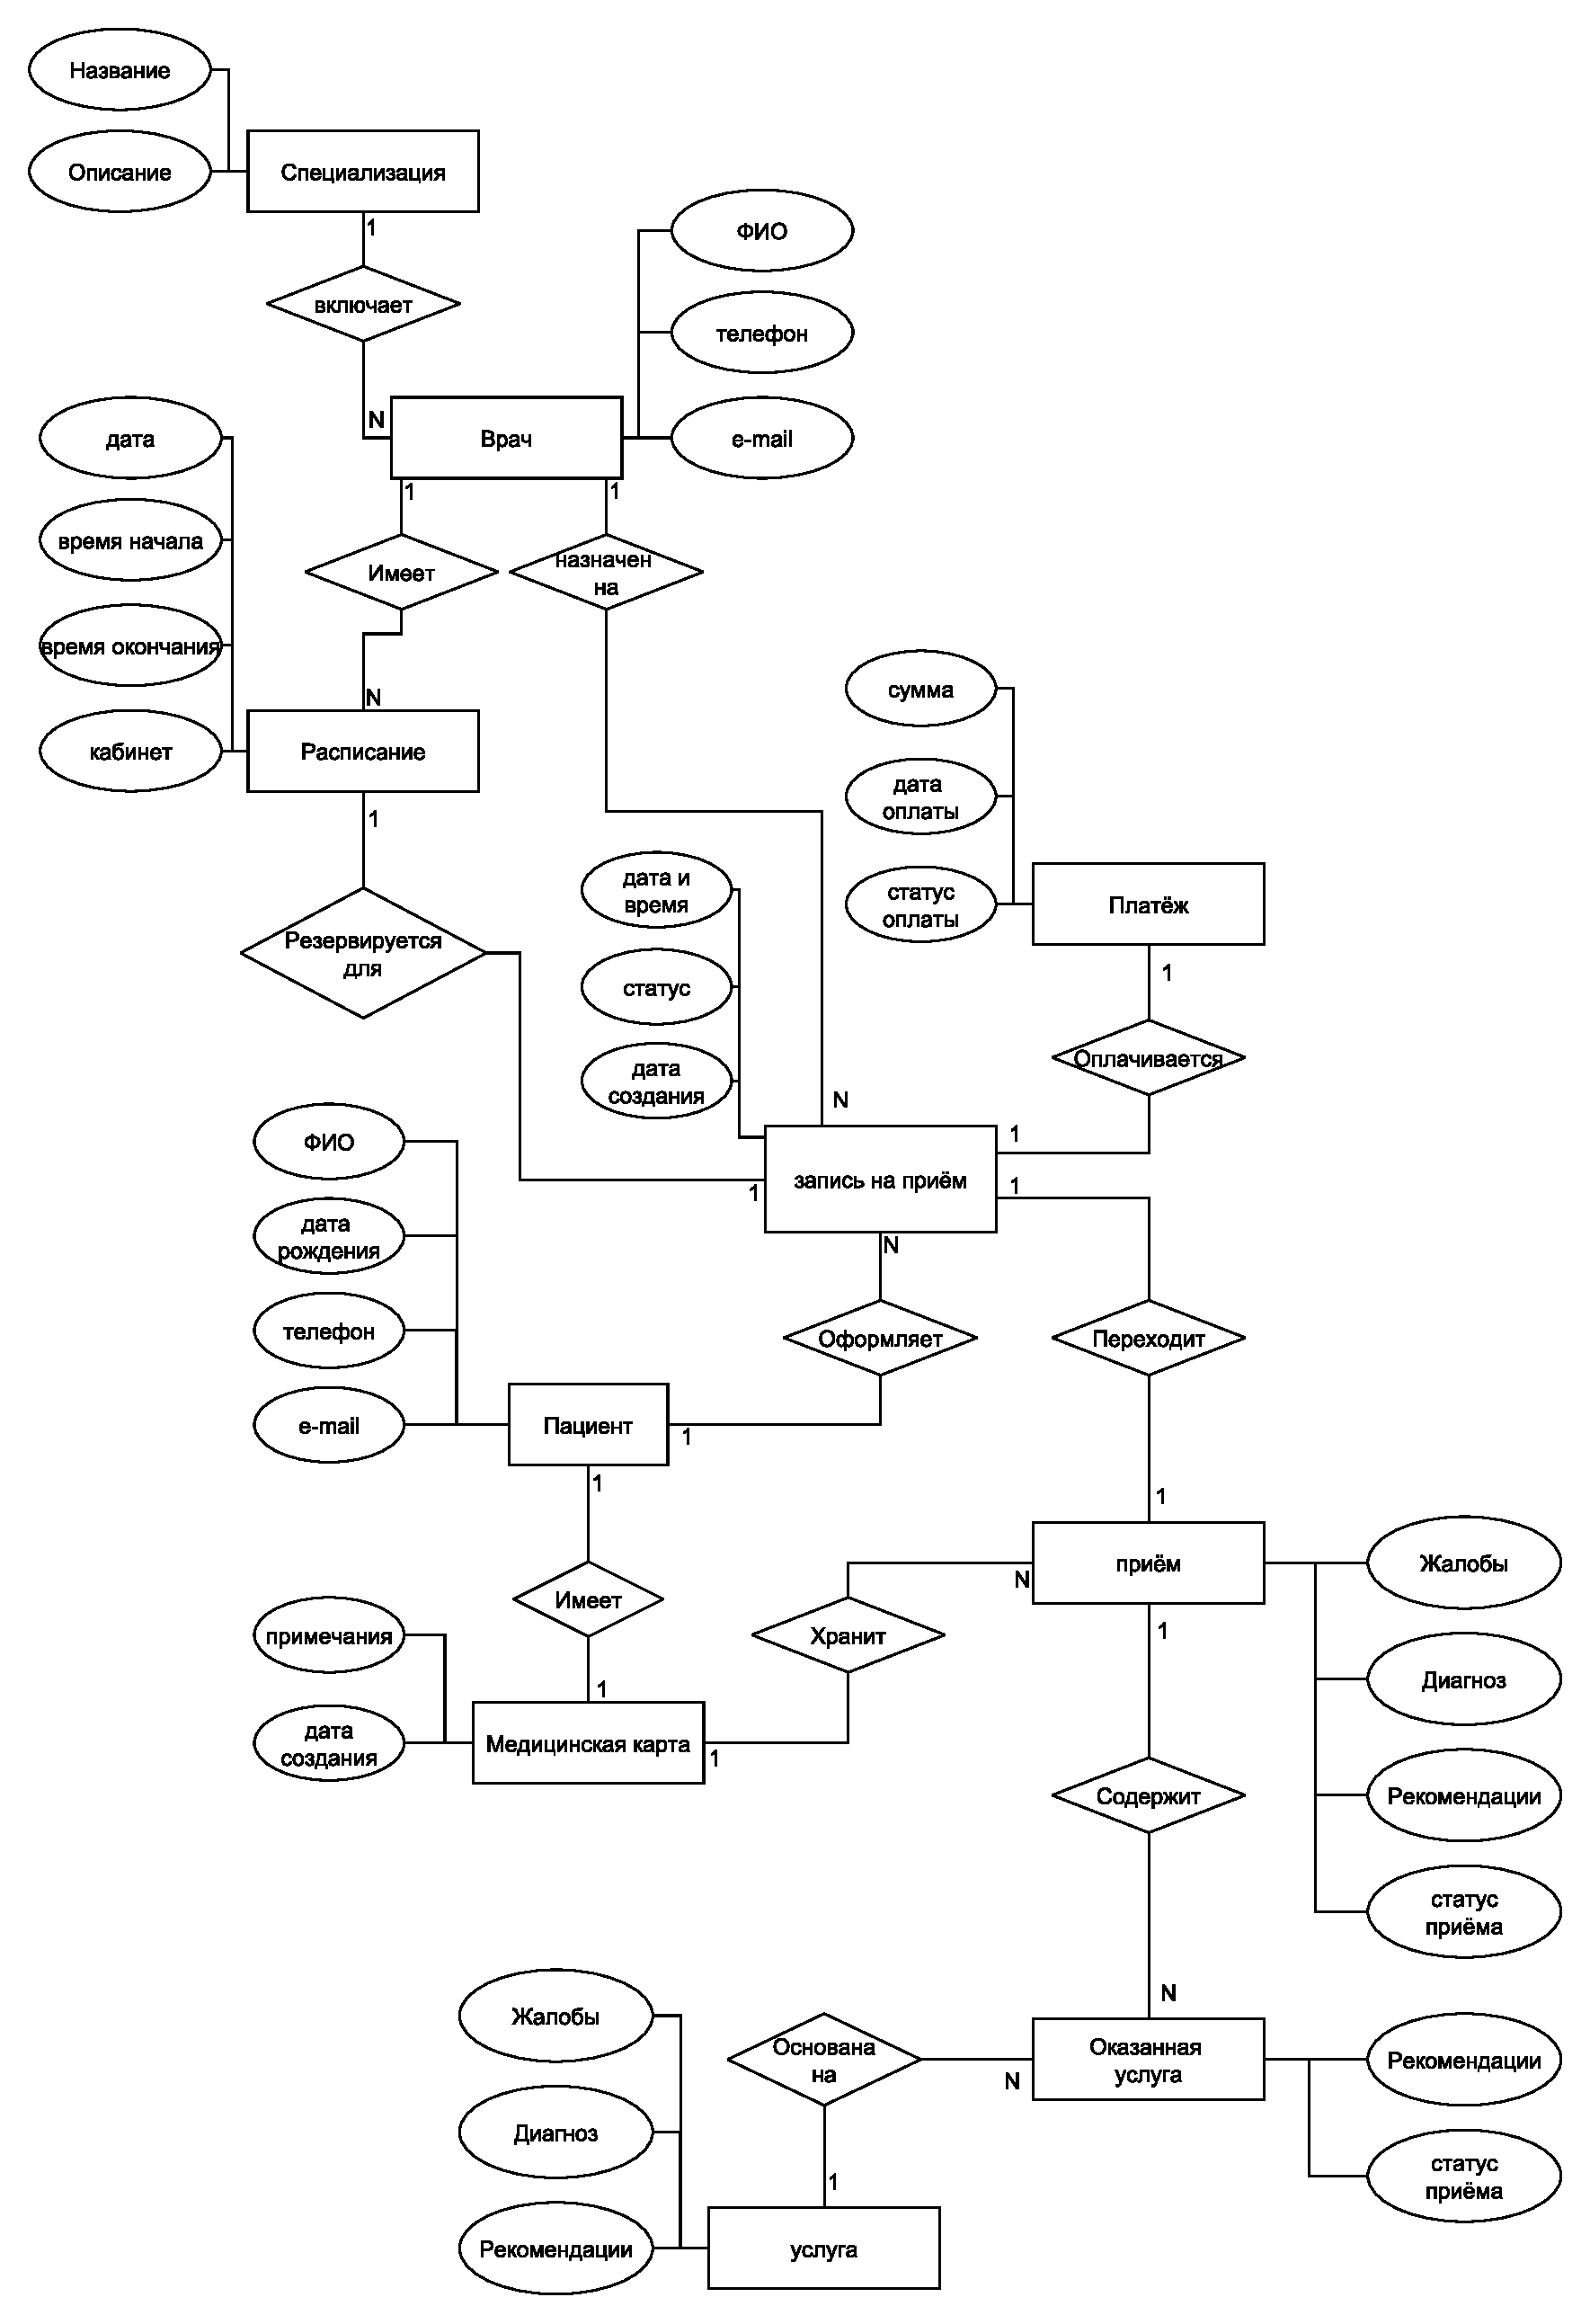
\includegraphics[width=\textwidth,height=0.80\textheight,keepaspectratio]{figures/er-diagram.pdf}
    \caption{ER-диаграмма сущностей базы данных медицинской клиники}
    \label{fig:er-diagram}
\end{figure}

Таким образом, база данных должна обслуживать не только хранение справочной информации, но и сквозной процесс оказания медицинской услуги: от записи пациента на прием до формирования счета и регистрации оплаты.

\section{Формализация ролей}

В системе выделяются три прикладные роли:
\begin{enumerate}
    \item пациент;
    \item администратор;
    \item врач.
\end{enumerate}

Для каждой роли определен собственный набор полномочий. Пациент регистрирует собственную карточку, выбирает врача и услугу, оформляет запись и при необходимости отменяет ее с учетом установленных ограничений. Администратор управляет пользователями, ролями, справочниками и финансовыми операциями, а также сопровождает запись пациента. Врач работает со своим расписанием, проводит прием и фиксирует его результаты.

Полномочия ролей приведены в таблице~\ref{tab:role-responsibilities}.

\begin{table}[ht]
    \centering
    \caption{Роли пользователей и их основные полномочия}
    \label{tab:role-responsibilities}
    \begin{tabular}{|p{3.2cm}|p{5.6cm}|p{4.7cm}|}
        \hline
        Роль & Основные действия & Ограничения \\
        \hline
        Пациент & регистрация собственной карточки, запись и отмена приема, просмотр доступного расписания и прайс-листа & не проводит прием, не регистрирует оплату и не управляет ролями \\
        \hline
        Администратор & управление пользователями, ролями, справочниками, просмотр счетов, регистрация оплат и сопровождение записи пациента & не проводит прием \\
        \hline
        Врач & просмотр своего расписания, завершение приема, фиксация диагноза и оказанных услуг & не регистрирует оплаты и не управляет пользователями \\
        \hline
    \end{tabular}
\end{table}

На рисунке~\ref{fig:use-case} приведена диаграмма вариантов использования, отражающая основные действия ролей в системе.

\begin{figure}[H]
    \centering
    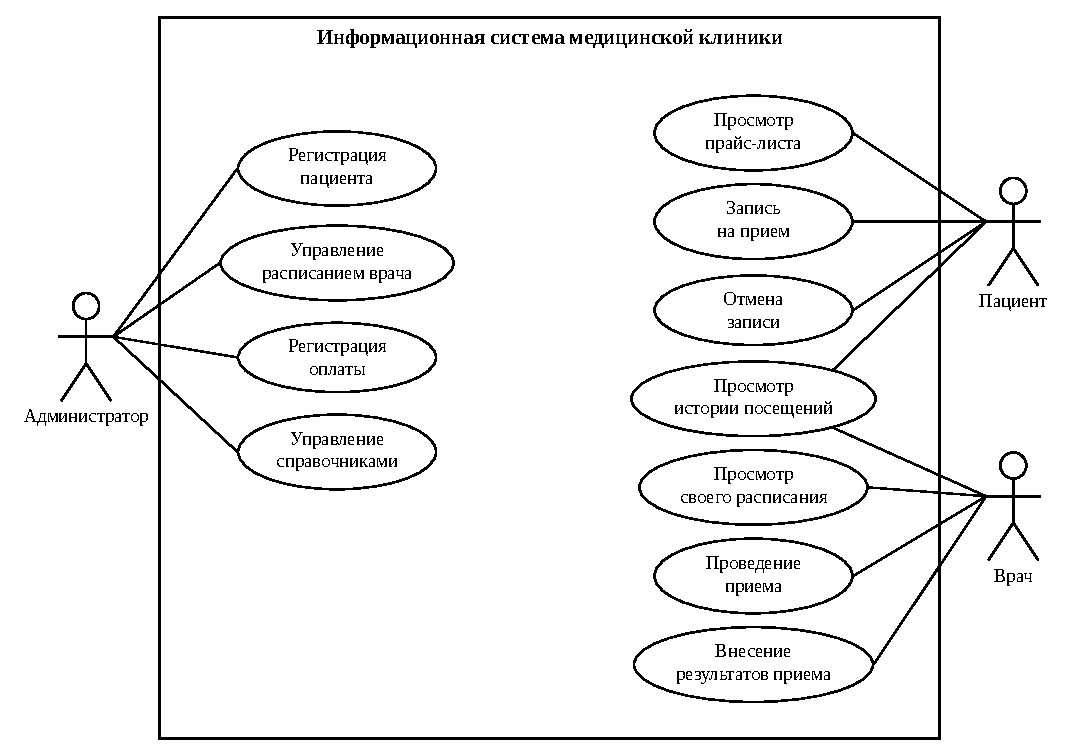
\includegraphics[width=\textwidth,height=0.80\textheight,keepaspectratio]{../diagrams/svg/use-case.pdf}
    \caption{Диаграмма вариантов использования системы медицинской клиники}
    \label{fig:use-case}
\end{figure}

Ролевая структура напрямую влияет на проектирование прикладного API и прав доступа в базе данных, поэтому в конструкторском разделе она будет детализирована уже в терминах ролей PostgreSQL и доступных операций.

\section{Модели данных}

\subsection{Иерархическая модель}

Иерархическая модель данных представляет базу как дерево, в котором каждая запись, кроме корневой, имеет единственного родителя~\cite{date_intro}. Классическим примером является СУБД IBM IMS, разработанная в 1960-х годах для хранения спецификаций космической программы Apollo. Запросы в иерархической модели выполняются навигационным способом --- путем обхода дерева от корня к потомкам.

Для предметной области медицинской клиники такой подход неудобен: пациент, врач, услуга, прием и счет образуют сеть взаимосвязанных сущностей, а не простую древовидную иерархию. Например, один пациент может иметь несколько записей к разным врачам, а один врач --- несколько услуг, что невозможно выразить единственным деревом без дублирования данных.

\subsection{Сетевая модель}

Сетевая модель, формализованная в стандарте CODASYL~\cite{connolly_db}, позволяет записи иметь несколько родительских и дочерних записей, что снимает ограничение иерархической модели. Примером является СУБД IDMS. Навигация по данным осуществляется через явные указатели между записями.

Однако проектирование и сопровождение сетевой модели значительно сложнее, а ее практическое применение в современных прикладных системах ограничено. Изменение структуры связей требует модификации схемы на физическом уровне, что делает модель негибкой для развивающейся системы клиники.

\subsection{Реляционная модель}

Реляционная модель, предложенная Э.\,Ф.~Коддом в 1970 году~\cite{date_intro}, хранит данные в виде отношений (таблиц), связанных между собой ключами. Она естественно поддерживает нормализацию, ограничения целостности, индексы, транзакции, представления, процедуры и триггеры~\cite{connolly_db}. Примеры современных реляционных СУБД: PostgreSQL, MySQL, Oracle Database, Microsoft SQL Server.

Для медицинской клиники это особенно важно, так как требуется одновременно обеспечить целостность расписания, истории цен, приемов, счетов и оплат. Декларативный язык SQL позволяет формулировать сложные запросы без навигационного обхода данных.

\subsection{Многомерная модель}

Многомерная модель ориентирована на аналитические и OLAP-задачи, когда данные рассматриваются как факты и измерения~\cite{connolly_db}. Типичная реализация --- куб данных с осями <<время>>, <<услуга>>, <<врач>>. Примеры СУБД: Microsoft Analysis Services, ClickHouse (колоночное хранение).

Для основной транзакционной системы клиники такая модель непригодна, поскольку операции записи, отмены, проведения приема и оплаты требуют именно оперативной обработки (OLTP) и строгих ограничений целостности, которые многомерные СУБД не обеспечивают.

\subsection{Объектно-ориентированная модель}

Объектно-ориентированная модель хранит данные в виде объектов с инкапсулированными методами и поддерживает наследование~\cite{date_intro}. Примерами являются СУБД ObjectDB и db4o. Такая модель удобна при тесной интеграции с объектными языками программирования.

Однако в рамках данной задачи она не дает достаточных преимуществ перед реляционной моделью. Контроль целостности временных интервалов (EXCLUDE-ограничения), кэширование и конкурентный доступ в курсовом проекте должны опираться на развитые возможности реляционной СУБД, которых объектно-ориентированные СУБД в полной мере не предоставляют.

\subsection{Выбор модели данных}

Сравнение рассмотренных моделей данных по критериям, существенным для разрабатываемой системы, приведено в таблице~\ref{tab:model-comparison}.

\begin{table}[ht]
    \centering
    \caption{Сравнение моделей данных}
    \label{tab:model-comparison}
    \small
    \begin{tabular}{|p{4.0cm}|c|c|c|c|c|}
        \hline
        Критерий & Иерарх. & Сетевая & Реляц. & Многомер. & ОО \\
        \hline
        Связи M:N & Нет & Да & Да & Нет & Да \\
        \hline
        Декларативные запросы & Нет & Нет & Да & Частично & Нет \\
        \hline
        Ограничения целостности & Частично & Частично & Да & Нет & Частично \\
        \hline
        Транзакционная обработка & Частично & Частично & Да & Нет & Да \\
        \hline
        Распространенность СУБД & Низкая & Низкая & Высокая & Средняя & Низкая \\
        \hline
    \end{tabular}
    \normalsize
\end{table}

Наиболее подходящей для разрабатываемой системы является реляционная модель данных. Она обеспечивает естественное выражение связей между сущностями, поддержку нормализации и надежную транзакционную обработку. Выбор PostgreSQL как реляционной СУБД~\cite{postgres_main} дополнительно позволяет использовать перечислимые типы, домены, диапазоны времени, ограничения \texttt{EXCLUDE}~\cite{postgres_constraints}, процедуры и триггеры, что полностью соответствует требованиям задания.

\section{Вывод}

В аналитическом разделе исследована предметная область медицинской клиники, формализована задача разработки базы данных и приложения, выделены сущности и роли пользователей, а также рассмотрены основные модели данных. По результатам анализа обоснован выбор реляционной модели и сформирована основа для конструкторского проектирования базы данных, процедур, ролевой модели и механизмов кэширования.

\clearpage
